\section{Main Questions in Neural Network Theory}
\label{sec:Question}
Neural Networks have unfolded a striking power processing human like
work. However, the mechanism underneath such success is beyond our 
comprehension. Center for Brains, Minds and Machines (CMBB) has done
plentiful work on giving a satisfying characterization of the deep 
neural networks and completing our understanding of deep neural networks.
In this section, we attend to three main questions put forward 
in Poggio et al. \parencite{poggio2016theory,poggio2017theory,
banburski2019theory}: (1) Why deep neural networks avoid the 
exponentially increasing computation
as the dimension increases comparing to shallow networks? 
(2) How does the landscape of the empirical risk looks like in 
the deep neural networks?


\subsection{Representation Power of Deep Neural Networks}
The main conclusion that Poggio et al. \parencite{poggio2016theory} 
draw is that for all compositional functions with binary tree 
architecture deep neural networks eliminate the dependency on 
variable dimensionality in complexity.

\subsubsection{Definition and Notation}
\textbf{Degree of approximation} Let $ V_N $ be a set of all networks
with complexity $ N $\footnote{The complexity we mean here is the 
total number of units in neural networks}, $ f $ be the target 
function and $ P $ be the approximation given by networks. 
Then the degree of approximation is:
\begin{equation}
    \mathop{\text{dist}}(f,\ V_N) = \mathop{\inf}_{P\in V_N}||f-P||
\end{equation}
If $ \mathop{\text{dist}}(f,\ V_N) = O(N^{\gamma}) $, then the complexity
$ N = O(\epsilon^{-\frac{1}{\gamma}}) $ can guarantee a approximation
with accuracy at least $ \epsilon $.

\textbf{Function set} Let $ m,\ n \geq 1,\ m \in Z $, then $ W_m^n $
is the set of all functions of $ n $ variables with continuous partial
derivatives of orders up to $ m $.
 $ W_m^{n,\ 2} \subseteq W_m^n $ is 
a set of all compositional functions of $ n $ variables with a binary
tree architecture i.e. using functions $ h \in W_m^2 $. 
Let $ k \in R^+ $ is the degree of a polynomial, then $ P_k^n $ is 
the set of all polynomial functions of degree $ k $ in $ n $ variables.
$ T_k^n $ is the set of all composition polynomials functions of degree 
$ k $ in $ n $ variables with a binary tree structure.

\subsubsection{Shallow Networks}
A theorem w.r.t. complexity of shallow network is stated in 
Mhaskar \parencite{mhaskar1996neural}.
\begin{thm}
    \label{thm:Shallow}
    Let activation $ \sigma $ be infinitely differentiable and not 
    a polynomial. For $ f \in W_m^n $, the complexity of shallow networks
    that provide accuracy at least $ \epsilon $ is:
    \begin{equation}
        N = O(\epsilon^{-\frac{n}{m}})
    \end{equation}
\end{thm}
The term $ \epsilon^{-\frac{n}{m}} $ shows the exponentially increasing
of neural network units in shallow networks.

\subsubsection{Deep Hierarchy Networks}
The second theorem is formulated in the binary tree structure see 
\autoref{fig:BT}. In CNN such structure corresponds to the $ 2\times 2 $
kernel.
\begin{thm}
    Let activation $ \sigma $ be infinitely differentiable and not 
    a polynomial. For $ f \in W_m^{n,\ 2} $, the complexity of shallow networks
    that provide accuracy at least $ \epsilon $ is:
    \begin{equation}
        N = O((n-1)\epsilon^{-\frac{2}{m}})
    \end{equation}
\end{thm}

\begin{prf}
    We apply \autoref{thm:Shallow} to $ h \in W_m^2 $, which means the
    approximation provides accuracy $ \epsilon = c_1N^{-\frac{m}{2}},\ c_1 \in R $.
    We illustrate the proof using a example of $ f(h_1,\ h_2),\ P(P_1,\ P_2) $.
    Since
    \begin{equation}
        \begin{split}
            ||f-P|| & \leq \epsilon \\
            ||h_1-P_1|| & \leq \epsilon \\
            ||h_2-P_2|| & \leq \epsilon \\            
        \end{split}
    \end{equation}
    Then we can derive:
    \begin{align}
        ||f(h_1,\ h_2) - P(P_1,\ P_2)|| & = ||f(h_1,\ h_2) - f(P_1,\ P_2) + f(P_1,\ P_2) - P(P_1,\ P_2)|| \\
        & \leq ||f(h_1,\ h_2) - f(P_1,\ P_2)|| + ||f(P_1,\ P_2) - P(P_1,\ P_2)|| \\
        & \leq c_2N^{-\frac{m}{2}}
    \end{align}
    Here we obtain the complexity of a single node in architecture, 
    despite the output node, we come to the conclusion of 
    $ N = O((n-1)\epsilon^{-\frac{2}{m}}) $. \\
    \textbf{Q.E.D.}
\end{prf}

\begin{figure}[H]
    \centering
    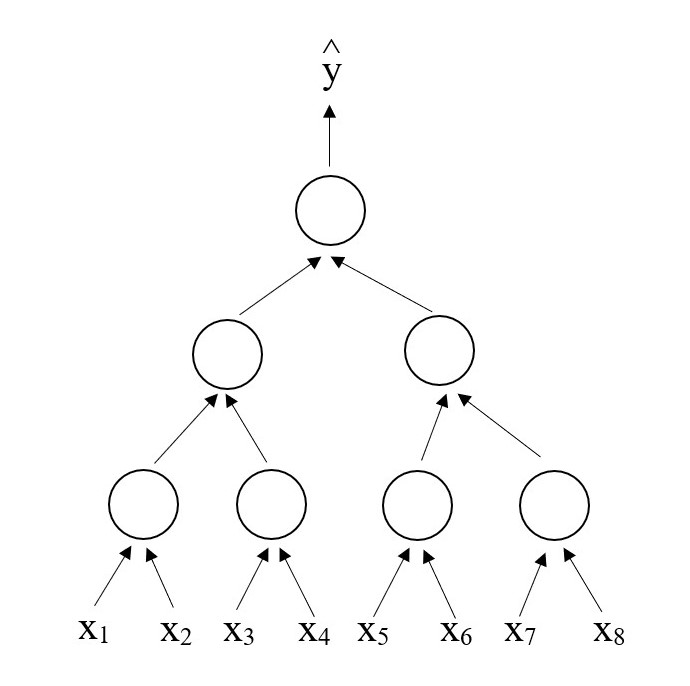
\includegraphics[width=8cm]{BT}
    \caption{\label{fig:BT}The binary tree structure}
\end{figure}


\subsection{The Landscape of Empirical Risk}
\label{ssec:empirical}
The term empirical risk is in contrast of the true risk, the average
loss on the true distribution over all input and output. The true 
distribution is unknown, otherwise there is no need for neural 
networks. Using data set, subset of the whole distribution, as 
substitution is the origin of empirical. Poggio et al. 
\parencite{poggio2017theory} explore the landscape of the empirical
risk, i.e. cost function $ J $, under the framework of convolutional
and overparameterized neural networks and the activation functions 
$ g^{[l]}(z) $ are polynomial-like ReLU\footnote{The ReLU is 
approximated by polynomials whose degree is $ d^{[l]}(\epsilon) $ at 
the accuracy of $ \epsilon $. }. Moreover, a landscape model satisfying
the experimental results is provided.

\par First, we summarize the experimental observations in deep neural
networks.
\begin{enumerate}
    \item There is a large number of zero-error global minimums 
    that are degenerate.\footnote{See Appendix 3 for
    theoretical analysis}
    \item Perturbation will lead to different convergence path, 
    the larger or earlier in training process the perturbation is,
    the more different the path and the final minimum will be.
    \item Interpolation between two close convergence path to the 
    same minimum will have similar or even smaller error. On the 
    other hand, interpolation between two minimums cause the 
    rise of error.
    \item No local minimum is observed.
\end{enumerate}



A simple model that is consistent with the observations is a collection
of rugged basins which is shown in \autoref{fig:Basin}. 
The flat and wide global minimums in basins explain
a myriad of zero-error minimizers. A small perturbation will not make 
a difference in a basin, while a lager one may cause a different path
to other basins, see \autoref{fig:basin}. Besides, the "walls" between
basins demonstrated in \autoref{fig:basin} may be the cause of 
interpolation's different behaviors in the neighbor of minimum and a
distinct minimum. 

\begin{figure}[H]
    \centering
    \subfigure[Profile view of the basin]{
        \begin{minipage}[t]{0.5\linewidth}
        \label{fig:Basin_1D}
        \centering
        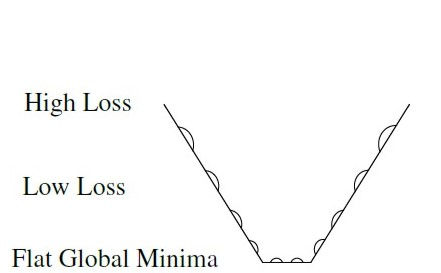
\includegraphics[width=6cm]{Basin_1D}
        \end{minipage}%
    }%
    \subfigure[Top-down view of the basin]{
        \begin{minipage}[t]{0.5\linewidth}
        \label{fig:Basin_2D}
        \centering
        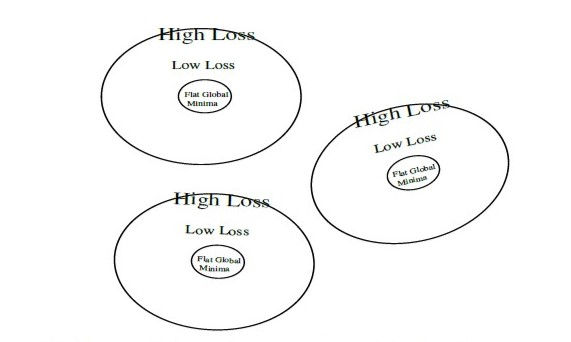
\includegraphics[width=6cm]{Basin_project}
        \end{minipage}%
    }%

    \subfigure[Example of perturbation]{
        \begin{minipage}[t]{0.5\linewidth}
        \label{fig:Basin_perturbation}
        \centering
        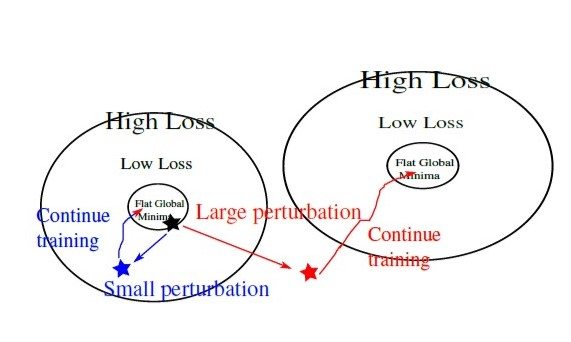
\includegraphics[width=6cm]{Basin_perturbation}
        \end{minipage}%
    }%
    \subfigure[Example of interpolation]{
        \begin{minipage}[t]{0.5\linewidth}
        \label{fig:Basin_interpolation}
        \centering
        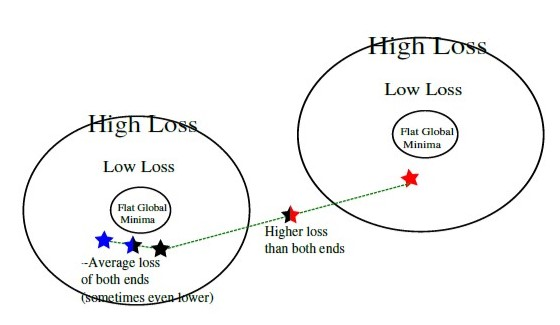
\includegraphics[width=6cm]{Basin_interpolation}
        \end{minipage}%
    }%
    \centering
    \caption{\label{fig:Basin}The basin model}
\end{figure}

Another interesting model is a variant of basin: the basin-fractal
\autoref{fig:Fractal}.
The key difference between simple basins and basin-fractal is that 
there are more than one global minimum in the same low loss area in 
the latter model. Though in most cases the "walls" between these 
global minimums are too flat and smooth to notice.

\begin{figure}[H]
    \centering
    \subfigure[2D view of basin-fractal]{
        \begin{minipage}[t]{0.5\linewidth}
        \centering
        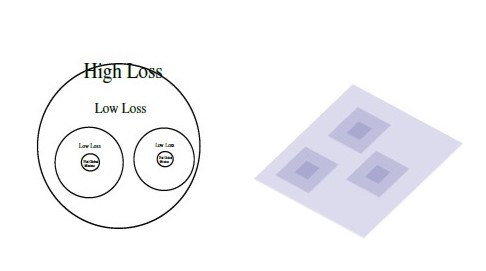
\includegraphics[width=6cm]{Fractal_project}
        \end{minipage}%
    }%
    \subfigure[The landscape of basin-fractal]{
        \begin{minipage}[t]{0.5\linewidth}
        \centering
        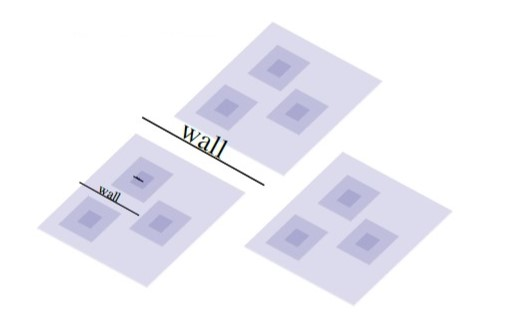
\includegraphics[width=6cm]{Fractal_landscape}
        \end{minipage}%
    }%
    \centering
    \caption{\label{fig:Fractal}The basin-fractal model}
\end{figure}





\subsection{Generalization of Neural Networks}
There is no use for neural networks only fit the training data 
well. The character of a neural network is measured by how well
it performs on other data, which is how well it generalizes.
Due to the obscurity of mathematical analysis in Banburski et al.
\parencite{banburski2019theory}, we only give a summary on 
the whole work.
\begin{enumerate}
    \item Using the exponential loss\footnote{The exponential loss
    is defined as $ l(y f)=e^{-y f} $, then the cost function is 
    $J(f)=\sum_{n=1}^{N} l\left(y_{n} f\left(x_{n}\right)\right)$} 
    , minimization of $ J $ with a vanishing regularization term in
    weights leads to the maximization of the margin of $f$.
    \item The critical points are hyperbolic equilibrium points\footnote{
    A hyperbolic equilibrium point is a point at which the Jacobian Matrix
    has no eigenvalue with zero real part.\parencite{hyperbolic}} if the 
    data are separable.
    
\end{enumerate}

